\documentclass[titlepage, 11pt]{article}
\usepackage[a4paper, total={6in, 9.5in}]{geometry}
\usepackage{graphicx}
\usepackage{amsmath,amsfonts,amssymb}
\usepackage{listings}
\usepackage{booktabs}
\usepackage[T1]{fontenc}
\usepackage{listings}
\usepackage{color}
\usepackage{minted}
\usepackage[colorlinks=true, linkcolor=blue, urlcolor=blue, citecolor=blue, pdfborder={0 0 255}]{hyperref}
\usepackage{colortbl}
\usepackage{url}
\usepackage{xcolor}
\usepackage{caption}
\usepackage{subcaption}
\usepackage{dirtytalk}
\usepackage[semicolon, round]{natbib}
\usepackage[ruled]{algorithm2e}
\usepackage{tabto}
\usepackage{gnuplottex}
\usepackage{avremu}
\usepackage{graphicx}
\graphicspath{ {./images/} }
\captionsetup[table]{skip=10pt}
\renewcommand{\vec}[1]{\mathbf{#1}}
\SetKwComment{Comment}{$\triangleright$\ }{}

\usepackage{tikz}
\usetikzlibrary{shapes.geometric, arrows}

\tikzstyle{startstop} = [rectangle, rounded corners, 
minimum width=4cm, 
minimum height=1cm,
text centered, 
draw=black, 
fill=red!30]

\tikzstyle{io} = [trapezium, 
trapezium stretches=true, % A later addition
trapezium left angle=70, 
trapezium right angle=110, 
minimum width=4cm, 
minimum height=1cm, text centered, 
draw=black, fill=blue!30]

\tikzstyle{process} = [rectangle, 
minimum width=4cm, 
minimum height=1cm, 
text centered, 
text width=4cm, 
draw=black, 
fill=orange!30]

\tikzstyle{decision} = [diamond, 
minimum width=4cm, 
minimum height=1cm, 
text centered, 
draw=black, 
fill=green!30]
\tikzstyle{arrow} = [thick,->,>=stealth]

\tikzstyle{comment}= [rectangle, 
minimum width=4cm, 
minimum height=1cm, 
align=left, 
draw=white]

% \hypersetup{%
% 	colorlinks=true,
% 	linkcolor=blue,
% 	linkbordercolor={0 0 1}
% }

% \renewcommand\lstlistingname{Algorithm}
% \renewcommand\lstlistlistingname{Algorithms}
% \def\lstlistingautorefname{Alg.}



\newcommand{\argmin}{\mathop{\mathrm{argmin}}}
\newcommand{\argmax}{\mathop{\mathrm{argmax}}}
\newcommand{\minimize}{\mathop{\mathrm{minimize}}}
\newcommand{\maximize}{\mathop{\mathrm{maximize}}}
\newcommand{\st}{\mathop{\mathrm{subject\,\,to}}}
\newcommand{\dist}{\mathop{\mathrm{dist}}}
\newcommand{\norm}[1]{\left\lVert#1\right\rVert}
\renewcommand{\vec}[1]{\mathbf{#1}}



\def\R{\mathbb{R}}
\def\E{\mathbb{E}}
\def\P{\mathbb{P}}
\def\S{\mathbb{S}}
\def\Cov{\mathrm{Cov}}
\def\Var{\mathrm{Var}}
\def\half{\frac{1}{2}}
\def\quat{\frac{1}{4}}
\def\sign{\mathrm{sign}}
\def\supp{\mathrm{supp}}
\def\th{\mathrm{th}}
\def\tr{\mathrm{tr}}
\def\dim{\mathrm{dim}}
\def\dom{\mathrm{dom}}


\title{
{EE2016: Microprocessor Lab} \\~\\
{\vlarge Experiment 7: Computations using Atmel Atmega8 AVR through Assembly Program Emulation}\\
}\author{Ajeet E S, EE22B086
    & Amogh Agrawal, EE22B087
}
\date{27 September, 2023}

\begin{document}
\maketitle
\setcounter{page}{0}
\tableofcontents
\listoflistings
\listoffigures
\newpage


\section{Aim}
To implement arithmetic and logical manipulation programs using Atmel Atmega8 microcontroller in assembly program emulation.

\section{Google Drive Link}
The link to the codes and screenshots for the Experiment are uploaded here:

\href{https://drive.google.com/drive/folders/1tgHh5Nvm8ZXyKFr0yHIerb5qJSfbOAkr?usp=sharing} {Code and Screenshots}


\section{Problem 1: Common 8-bit Mathematical Operations} 

\subsection{Problem Statement}
Given two 8-bit binary words (byte), compute the sum and product, store it in two separate registers.

\subsection{Approach}
We use the ADD directive to add two numbers. The Syntax of this command is:
\begin{minted}{asm}
ADD Rd,Rr
\end{minted}

This adds Rd and Rr, and stores the result in Rd. 
~\\
~\\
We use the MUL directive to add two numbers. The Syntax of this command is:
\begin{minted}{asm}
MUL Rd,Rr
\end{minted}

It multiplies both the numbers and stores the Lower byte in R0 and the Higher Byte in R1. These values are then extracted from there and stored in two consecutive registers

\subsection{Flowchart}

\begin{center}
\begin{tikzpicture}[node distance=2cm]

\node (start) [startstop] {Start};
\node (in1) [io, below of=start] {Input Numbers NUM1,NUM2};
%\node (copyto_R18) [process, below of=in1] {Copy value to register};
\node (add) [process, below of=in1] {Add the two numbers, store};
\node (multiply) [process, below of=add] {Multiply the two numbers};
\node (store_result) [process, below of=multiply] {Store result in 2 consecutive registers};
\node (stop) [startstop, below of=store_result] {Stop};

\draw [arrow] (start) -- (in1);
%\draw [arrow] (in1) -- (copyto_R18);
%\draw [arrow] (copyto_R18) -- (add);
%\draw [arrow] (add) -- node[anchor=east] {yes} (pro2a);
\draw [arrow] (in1) -- (add);
\draw [arrow] (add) -- (multiply);
\draw [arrow] (multiply) -- (store_result);
\draw [arrow] (store_result) -- (stop);


% Place comments below the blocks
\node [comment, right of=in1, xshift=3.5cm] {LDI R16, NUM1\\
LDI R17, NUM2\\
MOV R18, R16};
%\node [comment, right of=copyto_R18,xshift=3.5cm] {MOV R18, R16};
\node [comment, right of=add,xshift=3.5cm] {ADD R18, R17};
\node [comment, right of=multiply,xshift=3.5cm] {MUL R16, R17};
\node [comment, right of=store_result,xshift=3.5cm] {LDS R19, 0x00\\
LDS R20, 0x01};
% \node [comment, right of=process2, xshift=1.5cm] {Comment for Process 2};
% \node [comment, right of=process3, xshift=1.5cm] {Comment for Process 3};

\end{tikzpicture}
\end{center}

\subsection{Code}
The code used to perform addition and multiplication is given below:

{\renewcommand\fcolorbox[4][]{\textcolor{black}{\strut#4}}
\inputminted[breaklines,
 mathescape,
 linenos,
 numbersep=5pt,
 frame=single,
 numbersep=5pt,
 xleftmargin=0pt]{asm}{"Prob1.asm"}}
\captionof{listing}{Code to Add and Multiply two Numbers}

\subsection{Screenshots}

\begin{figure}[H]
  \centering
  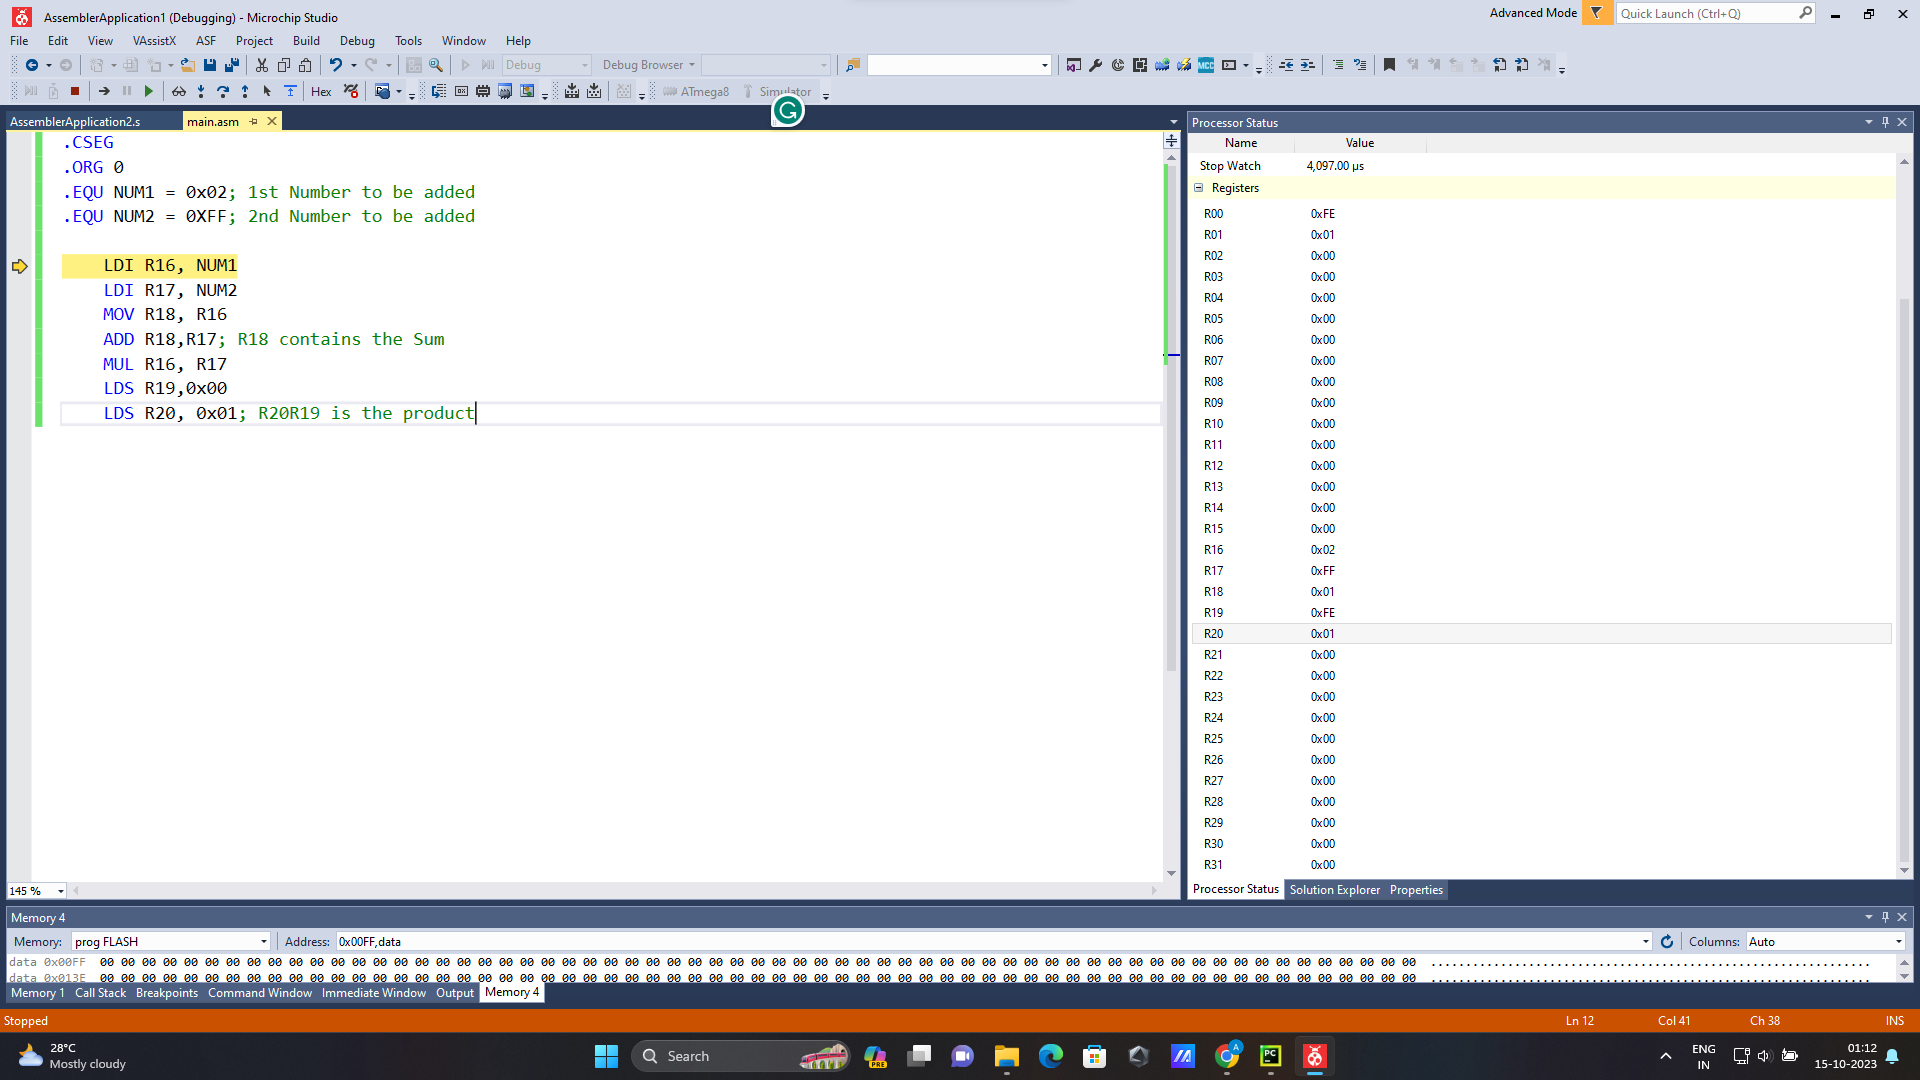
\includegraphics[width=1\linewidth]{prob1.png}
\end{figure}
\captionof{figure}{Screenshot for Problem 1}

\subsection{Inferences}
We infer there are in-built instructions for addition and multiplication in AVR.
\begin{minted}{asm}
ADD R17,R18
MUL R16, R17
\end{minted}

The MUL statement will store the multiplication contents in the R0 and R1 Registers.

\subsubsection{Register Transfers}
\begin{enumerate}
\item Load: Two LDI to initialise R16 and R17, Two LDI to store data to R19 and R20
\item Store: No Store has been done
\item Move: MOV to transfer data from R16 to R18
\end{enumerate}

\subsubsection{Clock Cycles per Instruction}
\begin{enumerate}
\item LDI: 1 Clock Cycle
\item MOV: 1 Clock Cycle
\item ADD: 1 Clock Cycle
\item MUL: 2 Clock Cycles
\item LDS: 2 Clock Cycles
\end{enumerate}

\subsubsection{Latency}
The latency of this AVR Assembly Code is $10 \mu s$

\subsubsection{Throughput}
Throughput of a code is defined as:
$$ Throughput \equiv \frac{\text{Number of Computations(tasks) Done}}{\text{Time Taken}}$$
Here, we define the task to be the number of (Addition+ Multiplication) per unit time

$Throughput= \frac{1}{10\mu s}=10^{5}$ Tasks /s

\subsubsection{Limitations}
\begin{enumerate}
\item This code can only add and multiply 8-bit numbers
\end{enumerate}


\section{Problem 2: Implementing Division on AVR}

\subsection{Problem Statement}
AVR has no division operation. Implement a code that takes the dividend from memory location A at 0x0E and the divisor from memory location B at 0x10. Note that these locations are not consecutive. You need to set the locations yourself. The TA would enter random numbers at these memory locations. Store the quotient in location 0xF0 and remainder in location 0xFF. For the sake of simplicity, assume that you are implementing unsigned division. (If you identify more than one algorithm for division, you can compute the difference in computational latency between the two).

\subsection{Approach}
The code takes values from the memory locations mentioned (Here, we have added code to write data onto those memory locations for demonstration purposes). Then, we perform repetitive subtraction of the divisor from the dividend in place until divisor>dividend while incrementing the quotient(stored in another register). At this point, the register containing the dividend will contain the remainder, and the quotient register will contain the quotient. These are then moved into the specified memory locations.

\subsection{Flowchart}
\begin{center}
\begin{tikzpicture}[node distance=2cm]

\node (start) [startstop] {Start};
\node (in1) [io, below of=start] {Take inputs, set Quotient=0};
\node (compare) [decision, below of=in1,yshift=-1.5cm] {Dividend $\leq$ Divisor};
\node (subtract_divisor) [process,below of = compare,yshift=-2cm] {Subtract Divisor from Dividend};
\node (add) [process, left of=compare,xshift=-3.5cm] {Increment Quotient};
\node (store_result) [process, right of=compare,xshift=3.5cm] {Store Quotient and Remainder};
\node (stop) [startstop, below of=store_result] {Stop};

\draw [arrow] (start) -- (in1);
\draw [arrow] (in1) -- (compare);
\draw [arrow] (compare) -- node[anchor=north] {No} (subtract_divisor);
% %\draw [arrow] (add) -- node[anchor=east] {yes} (pro2a);
% %\draw [arrow] (add) -- node[anchor=east] {yes} (pro2a);
\draw [arrow] (subtract_divisor) -| (add);
\draw [arrow] (add) -- (compare);
\draw [arrow] (compare) -- node[anchor=east] {Yes} (store_result);
\draw [arrow] (store_result) -- (stop);


% % Place comments below the blocks
% \node [comment, right of=in1, xshift=3.5cm] {LDI R16, NUM1\\
% LDI R17, NUM2\\
% MOV R18, R16};
% %\node [comment, right of=copyto_R18,xshift=3.5cm] {MOV R18, R16};
% \node [comment, right of=add,xshift=3.5cm] {ADD R18, R17};
% \node [comment, right of=multiply,xshift=3.5cm] {MUL R16, R17};
% \node [comment, right of=store_result,xshift=3.5cm] {LDS R19, 0x00\\
% LDS R20, 0x01};
% % \node [comment, right of=process2, xshift=1.5cm] {Comment for Process 2};
% % \node [comment, right of=process3, xshift=1.5cm] {Comment for Process 3};

\end{tikzpicture}
\end{center}

\subsection{Code}
The code used to perform division is given below:

{\renewcommand\fcolorbox[4][]{\textcolor{black}{\strut#4}}
\inputminted[breaklines,
 mathescape,
 linenos,
 numbersep=5pt,
 frame=single,
 numbersep=5pt,
 xleftmargin=0pt]{asm}{"Prob2.asm"}}
\captionof{listing}{Code to Perform Division}

\subsection{Screenshots}
\begin{figure}[H]
  \centering
  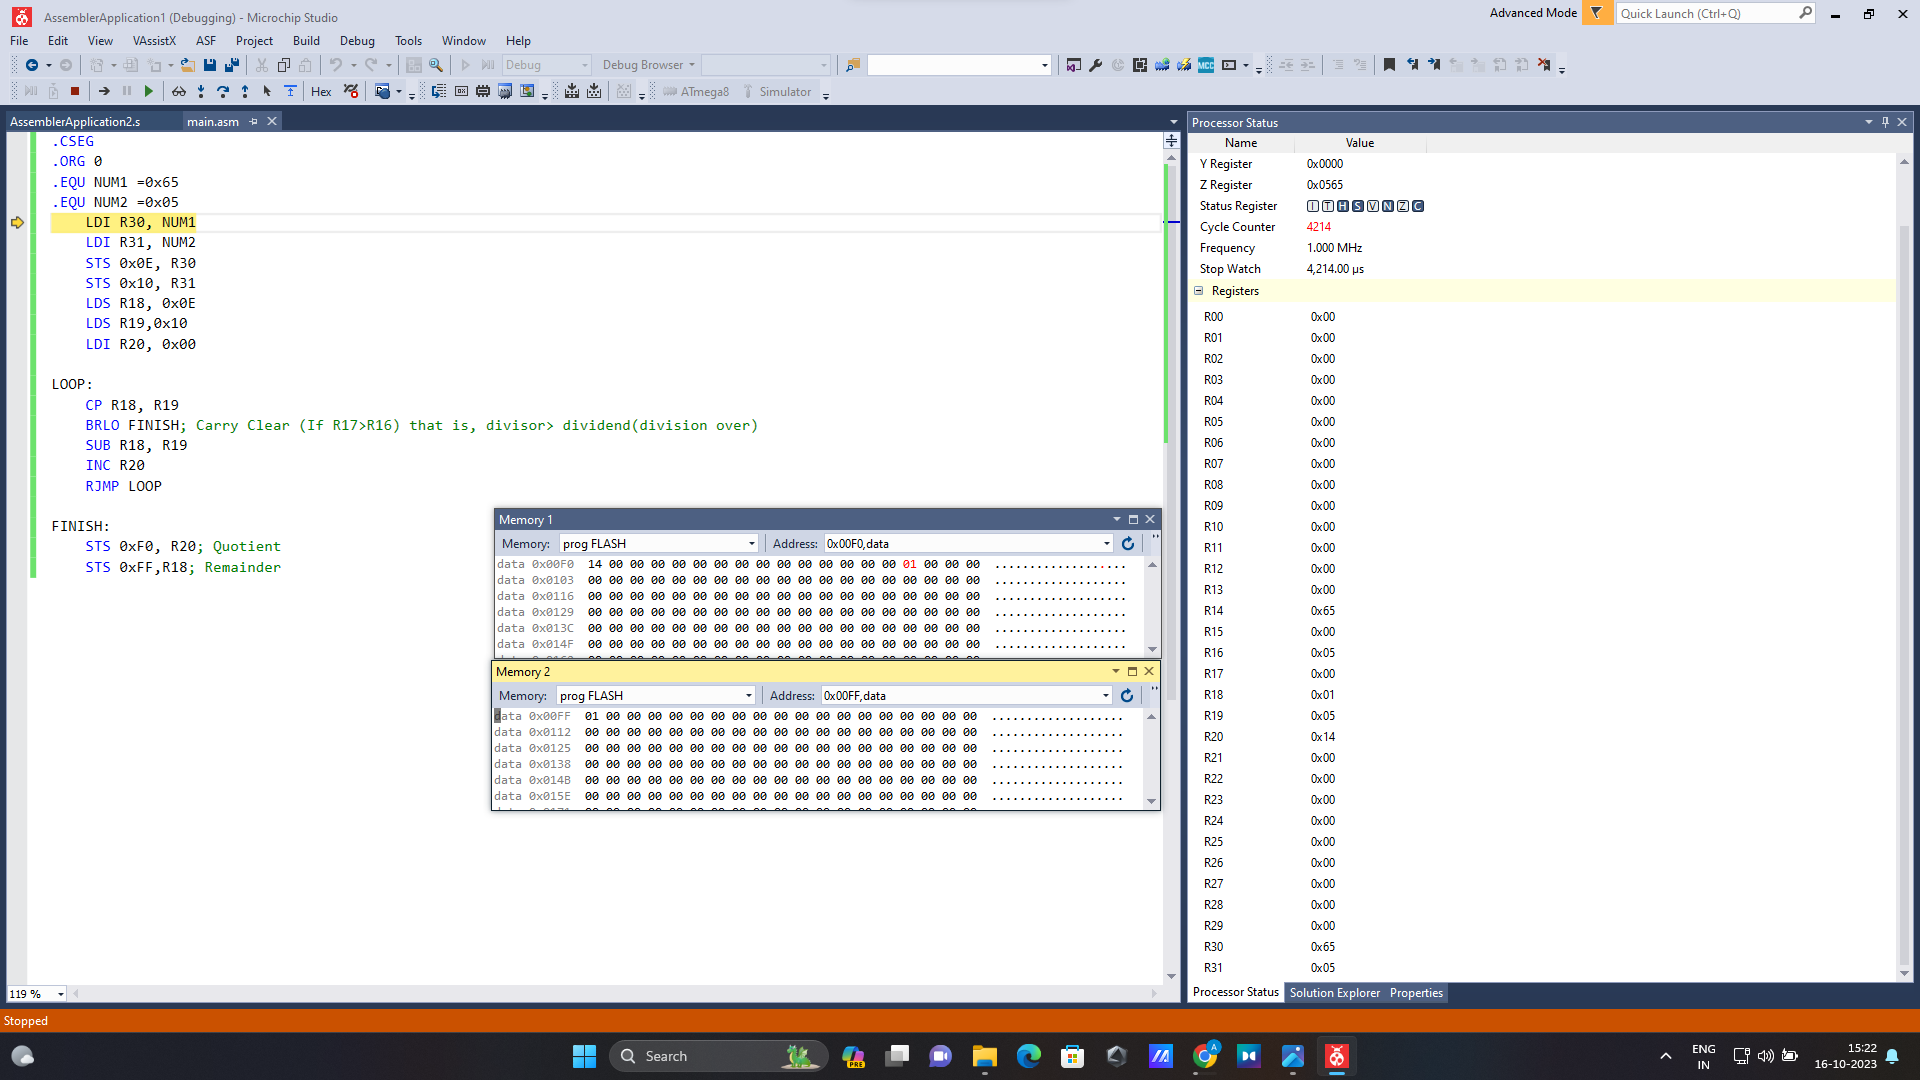
\includegraphics[width=1\linewidth]{prob2.png}
\end{figure}
\captionof{figure}{Screenshot for Problem 2}

\subsection{Inferences}
This assembly code is designed to perform integer division of two numbers, with NUM1 as the dividend and NUM2 as the divisor. The code calculates the quotient and remainder of the division and stores the results in memory locations 0xF0 (for quotient) and 0xFF (for remainder).

Since no in-built function exists, we use the continuous subtraction method to calculate the quotient and remainder.

\subsubsection{Register Transfers}
\begin{enumerate}
\item Load: LDI, LDS to load data
\item Store: STS to store
\item Move: SUB- Register to Register Moves
\end{enumerate}

\subsubsection{Clock Cycles per Instruction}
\begin{enumerate}
\item LDI: 1 Clock Cycle
\item MOV: 1 Clock Cycle
\item ADD: 1 Clock Cycle
\item MUL: 2 Clock Cycles
\item LDS: 2 Clock Cycles
\item STS: 2 Clock Cycles
\item CP: 1 Clock Cycle
\item INC: 1 Clock Cycle
\item RJMP: 2 Clock Cycles
\item Branch Statements: 1 or 2 Clock Cycles depending on result
\end{enumerate}

\subsubsection{Latency}
The latency of this AVR Assembly Code is $11 +6 \lfloor \frac{Divident}{Divisor} \rfloor + 7 \mu s$

\subsubsection{Throughput}
Throughput of a code is defined as:
$$ Throughput \equiv \frac{\text{Number of Computations(tasks) Done}}{\text{Time Taken}}$$
Here, we define the task to be the number of Divisions per unit time

$Throughput= \frac{10^{6}}{18 +6 \lfloor \frac{Divident}{Divisor} \rfloor} $ Tasks /s

\subsubsection{Limitations}
\begin{enumerate}
\item This code can only divide an unsigned 8-bit number by another unsigned 8-bit number
\end{enumerate}

\section{Problem 3: Parity Detection}
\subsection{Problem Statement}
Given an 8-bit number stored in location 0xFF, generate the odd parity of this number and store it at memory location 0xF0.

\subsection{Approach}
For this problem, if we have an 8-bit number, we divide it into two 4-bit numbers, take xor and then divide the next 4 bits into two two-bit numbers and continue this process until we get a single bit. This single bit is the odd parity.

\subsection{Flowchart}
\begin{center}
\begin{tikzpicture}[node distance=2cm]

\node (start) [startstop] {Start};
\node (in1) [io, below of=start] {Take Input};
\node (extract1) [process,below of = in1] {Extract the highest and lowest nibbles to R16,R17};
\node (xor1) [process, below of=extract1] {XOR R16, R17};
\node (extract2) [process,below of = xor1] {Extract the highest and lowest 2 bits of result to R30,R31};
\node (xor2) [process, below of=extract2] {XOR R30, R31};
\node (extract3) [process,below of = xor2] {Extract the highest and lowest bits of result to R16,R17};
\node (store_result) [process, below of=extract3] {XOR R16, R17; store the result};
\node (stop) [startstop, below of=store_result] {Stop};

\draw [arrow] (start) -- (in1);
\draw [arrow] (in1) -- (extract1);
\draw [arrow] (extract1) -- (xor1);
\draw [arrow] (xor1) -- (extract2);
\draw [arrow] (extract2) -- (xor2);
\draw [arrow] (xor2) -- (extract3);
\draw [arrow] (extract3) -- (store_result);
\draw [arrow] (store_result) -- (stop);


% % Place comments below the blocks
% \node [comment, right of=in1, xshift=3.5cm] {LDI R16, NUM1\\
% LDI R17, NUM2\\
% MOV R18, R16};
% %\node [comment, right of=copyto_R18,xshift=3.5cm] {MOV R18, R16};
% \node [comment, right of=add,xshift=3.5cm] {ADD R18, R17};
% \node [comment, right of=multiply,xshift=3.5cm] {MUL R16, R17};
% \node [comment, right of=store_result,xshift=3.5cm] {LDS R19, 0x00\\
% LDS R20, 0x01};
% % \node [comment, right of=process2, xshift=1.5cm] {Comment for Process 2};
% % \node [comment, right of=process3, xshift=1.5cm] {Comment for Process 3};

\end{tikzpicture}
\end{center}


\subsection{Code}
The code used to find the odd parity of a given 8-bit number is given below:

{\renewcommand\fcolorbox[4][]{\textcolor{black}{\strut#4}}
\inputminted[breaklines,
 mathescape,
 linenos,
 numbersep=5pt,
 frame=single,
 numbersep=5pt,
 xleftmargin=0pt]{asm}{"Prob3.asm"}}
\captionof{listing}{Code to Generate Odd Parity}

\subsection{Screenshots}
\begin{figure}[H]
  \centering
  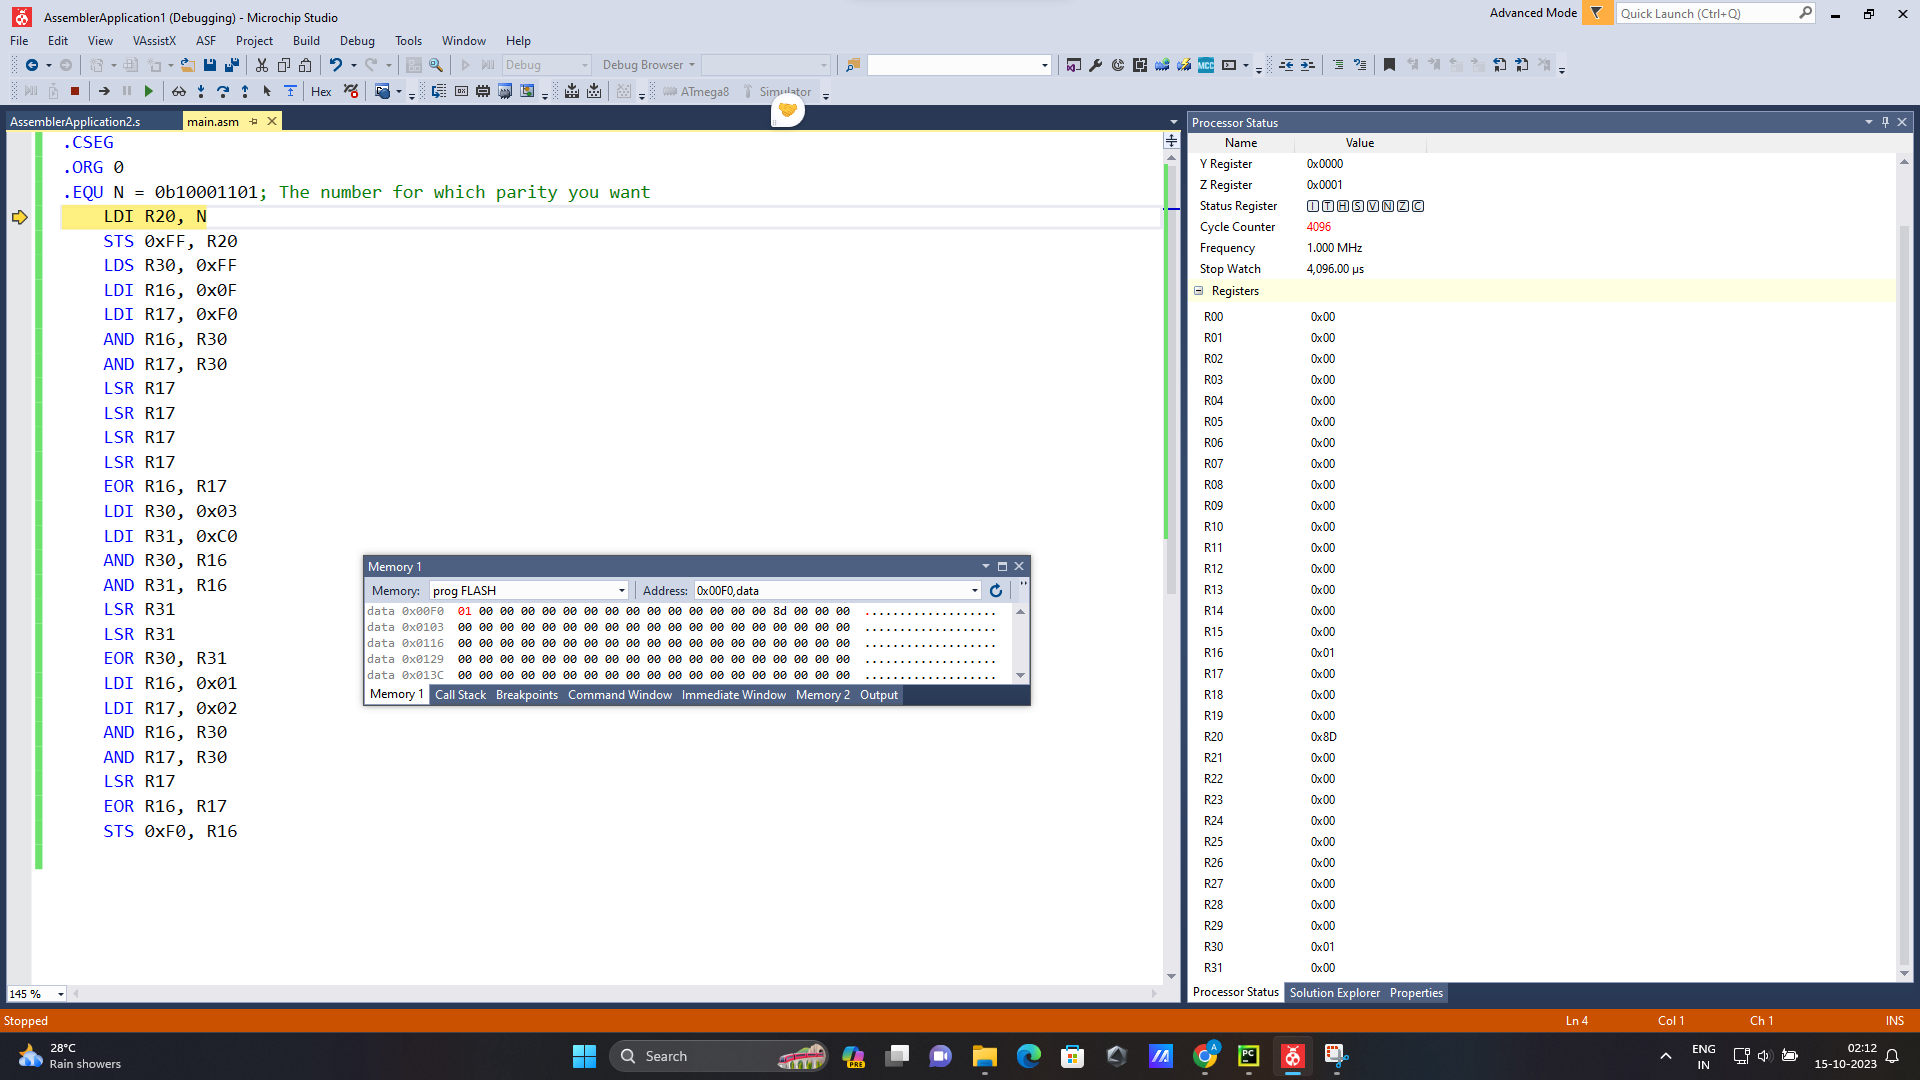
\includegraphics[width=1\linewidth]{prob3.png}
\end{figure}
\captionof{figure}{Screenshot for Problem 3}

\subsection{Inferences}
This assembly code calculates the odd parity of the binary number N to be input by the TA and stores the result in memory location 0xF0.
We infer from this that parity generation is essential since the data we get may be incorrect.

\subsubsection{Register Transfers}
\begin{enumerate}
\item Load: LDI, LDS to load data
\item Store: STS to store
\item Move: SUB- Register to Register Moves
\end{enumerate}

\subsubsection{Clock Cycles per Instruction}
\begin{enumerate}
\item LDI: 1 Clock Cycle
\item LDS: 2 Clock Cycles
\item STS: 2 Clock Cycles
\item LSR: 1 Clock Cycle
\item EOR: 1 Clock Cycle
\item AND: 1 Clock Cycle
\end{enumerate}

\subsubsection{Latency}
The latency of this AVR Assembly Code is $ 29 \mu s$

\subsubsection{Throughput}
Throughput of a code is defined as:
$$ Throughput \equiv \frac{\text{Number of Computations(tasks) Done}}{\text{Time Taken}}$$
Here, we define the task to be finding the Parity of the given number

$Throughput= \frac{1}{29 \mu s} =3.44 \times 10^{4}$ Tasks /s

\subsubsection{Limitations}
\begin{enumerate}
\item This code can only find the parity of an 8- bit number
\end{enumerate}

\section{Problem 4: Largest and Smallest of a number set given}
\subsection{Problem Statement}
Given a finite set of binary words, identify the largest and smallest number in the given set and store it at 0xF0 and 0xFF, respectively. Note that the TA will enter the finite set. You are supposed to develop a code that works for an arbitrary number of numbers.

\subsection{Approach}
For this problem, we first ask the TA's to store the set of values at the end of the program with the db tag. Then, the Values are taken one by one through the Z register, and this process is terminated if we get two consecutive 0xFF. While loop in through the Z register we keep on updating the max and the min value.

\subsection{Flowchart}

\begin{center}
\begin{tikzpicture}[node distance=2cm]

% Nodes
\node (start) [startstop] {Start};
\node (init1) [process, below of=start] {Initialize R25=0xFF, R20=0x00, Z to memory address of Words};
\node (load1) [process, below of=init1] {Load Consecutive Values to R17 and R18};
\node (checkifeq1) [decision, below of=load1, yshift=-2cm] {If R17 and R18 = 0xFF};
\node (update_highest) [process, below of=checkifeq1,yshift=-2.5cm] {Update existing highest value in R20, comparing with R17 and/or R18};

\node (init2) [process, right of=init1,xshift=5cm] {Initialize R21=0x00, Z to memory address of Words};
\node (load2) [process, right of=load1,xshift=5cm] {Load Consecutive Values to R17 and R18};
\node (checkifeq2) [decision, right of=checkifeq1, xshift=5cm,yshift=-0.5cm] {If R17 and R18 = 0xFF};
\node (update_lowest) [process, below of=checkifeq2,yshift=-2.7cm] {Update existing lowest value in R21, comparing with R17 and/or R18};
\node (store) [process, right of=checkifeq2,xshift=3.5cm] {Store Max and Min Values};
\node (stop) [startstop, below of=store] {Stop};

% Arrows
\draw [arrow] (start) -- (init1);
\draw [arrow] (init1) -- (load1);
\draw [arrow] (load1) -- (checkifeq1);
\draw [arrow] (checkifeq1) -- node[anchor=south] {No} (update_highest);
\draw [arrow] (update_highest) -| node[anchor=west] {} ++  (-2.5cm,0) |- (load1);

\draw [arrow] (checkifeq1) -| node[anchor=east] {Yes} ++  (3cm,0) |- (init2);
\draw [arrow] (init2) -- (load2);
\draw [arrow] (load2) -- (checkifeq2);
\draw [arrow] (update_lowest) -| node[anchor=west] {} ++  (-2.7cm,0) |- (load2);
\draw [arrow] (checkifeq2) -- node[anchor=east] {Yes} (store);
\draw [arrow] (checkifeq2) -- node[anchor=south] {No} (update_lowest);
\draw [arrow] (store) -- (stop);
% \draw [arrow] (number) -- (update);
% \draw [arrow] (update) -- node[anchor=east] {Yes} (loop);
% \draw [arrow] (loop) -- (next);
% \draw [arrow] (update) -| node[anchor=east] {No} ++(-2cm,0) |- (loop);
% \draw [arrow] (next) -- (number1);
% \draw [arrow] (number1) -- (update1);
% \draw [arrow] (update1) -- node[anchor=east] {Yes} (loop1);
% \draw [arrow] (loop1) -- (exit);
% \draw [arrow] (update1) -| node[anchor=east] {No} ++(-2cm,0) |- (loop1);

\end{tikzpicture}
\end{center}

\subsection{Code}
{\renewcommand\fcolorbox[4][]{\textcolor{black}{\strut#4}}
\inputminted[breaklines,
 mathescape,
 linenos,
 numbersep=5pt,
 frame=single,
 numbersep=5pt,
 xleftmargin=0pt]{asm}{"Prob4.asm"}}
\captionof{listing}{Code to Find the Largest and Smallest Number from a Given Set of Numbers}

\subsection{Screenshots}
\begin{figure}[H]
  \centering
  % include second image
  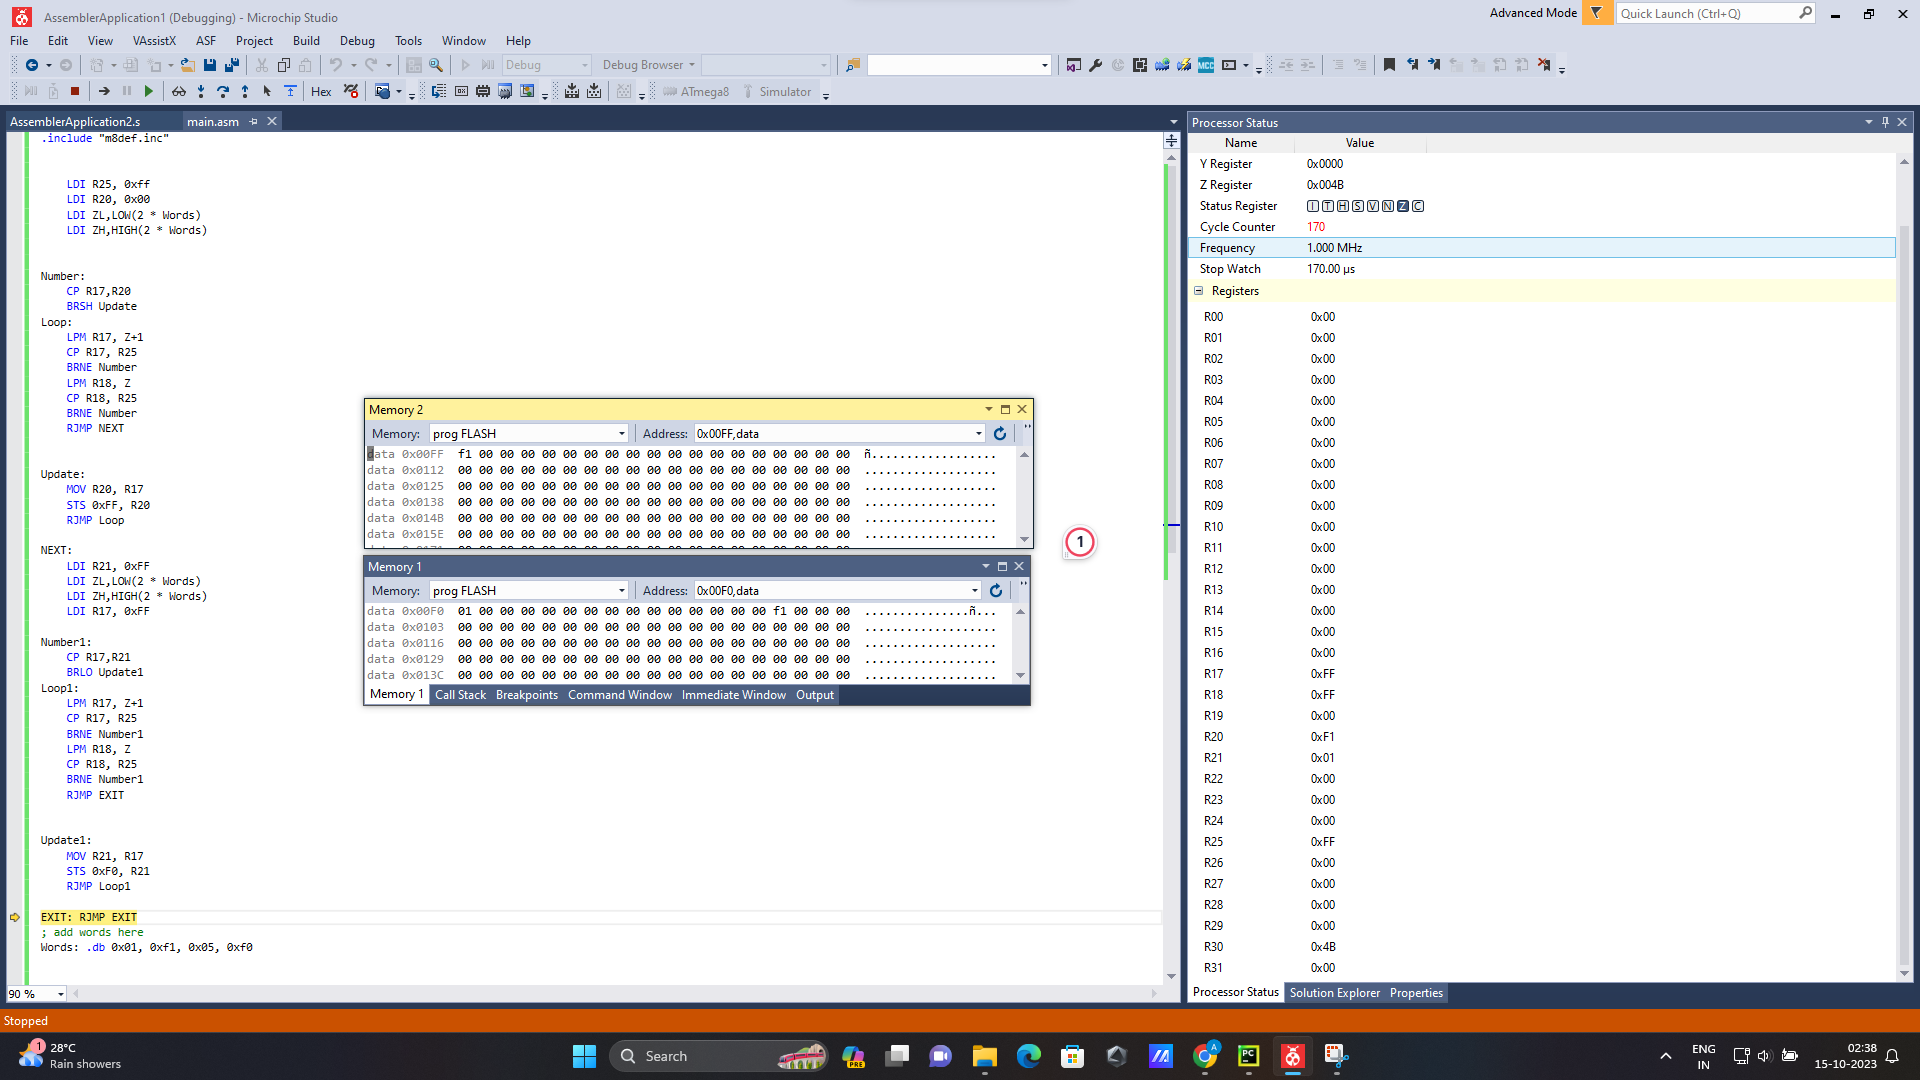
\includegraphics[width=1\linewidth]{prob4.png}
  \label{fig:B}
\end{figure}
\captionof{figure}{Screenshot for Problem 4}
\subsection{Inferences}

\subsubsection{Register Transfers}
\begin{enumerate}
\item Load: LDI, LDS to load data
\item Store: STS to store
\item Move: SUB- Register to Register Moves
\end{enumerate}

\subsubsection{Clock Cycles per Instruction}
\begin{enumerate}
\item LDI: 1 Clock Cycle
\item CP: 1 Clock Cycle
\item Branch Statements: 1 or 2 Clock Cycles depending on result
\item LPM: 3 Clock Cycles
\item RJMP: 2 Clock Cycles
\item MOV: 1 Clock Cycle
\item LDS: 2 Clock Cycles
\item STS: 2 Clock Cycles
\end{enumerate}

\subsubsection{Limitations}
\begin{enumerate}
\item This code cannot find maximum or minimum of the set of numbers if there are two or more repeating 0xFF. The code will not check further if that occurs.
\item The numbers being compared are assumed to be 8-bit numbers.
\end{enumerate}

\section{Problem 5: Fibonacci Sequence} 
\subsection{Problem Statement}
The Fibonacci sequence is a sequence of numbers that follows the recurrence $a(n+1) =a(n) + a (n-1)$ $\forall$ $n > 2$. The initial two terms of the sequence are $a (1) = 0$ and $a (2) = 1$. Given a number $N$ , calculate the $N^{th}$ term of the Fibonacci sequence $a(N)$ and store it in register $R0$

\subsection{Approach}
For this program, we ask the TA first to input the Nth value of the Fibonacci series they want. Using this, we then calculate the values of all the Fibonacci series till the Nth value and store the Nth value in a memory location. This is done progressively by shifting the values of two temporary registers to the (N-1)Th and (N-2)Th values.

\subsection{Flowchart}
\begin{center}
\begin{tikzpicture}[node distance=2cm]

\node (start) [startstop] {Start};
\node (in1) [io, below of=start] {Take input N};
\node (initialise) [process, below of=in1] {Set R16=a(1),R17=a(2)\\
counter=N-1};
\node (next_element) [process, below of=initialise] {Set R16=R17,\\
R17=R16+R17};
\node (decrement_counter) [process, below of=next_element] {counter$--$};
\node (compare) [decision, below of=next_element,yshift=-3cm] {If counter $=$ 0};
\node (store_result) [process, below of=compare,yshift=-1cm] {Store Result};
\node (stop) [startstop, below of=store_result] {Stop};

\draw [arrow] (start) -- (in1);
\draw [arrow] (in1) -- (initialise);
\draw [arrow] (initialise) -- (next_element);
\draw [arrow] (next_element) -- (decrement_counter);
\draw [arrow] (compare) -- node[anchor=south] {Yes} (store_result);
\draw [arrow] (decrement_counter) -- (compare);
% %\draw [arrow] (add) -- node[anchor=east] {yes} (pro2a);
% %\draw [arrow] (add) -- node[anchor=east] {yes} (pro2a);
% \draw [arrow] (compare) -| node[anchor=east] {No} (next_element);
\draw [arrow] (compare) -- ++ (-4cm,0) |- node[anchor=west] {No} (next_element) ;

\draw [arrow] (store_result) -- (stop);


% % Place comments below the blocks
% \node [comment, right of=in1, xshift=3.5cm] {LDI R16, NUM1\\
% LDI R17, NUM2\\
% MOV R18, R16};
% %\node [comment, right of=copyto_R18,xshift=3.5cm] {MOV R18, R16};
% \node [comment, right of=add,xshift=3.5cm] {ADD R18, R17};
% \node [comment, right of=multiply,xshift=3.5cm] {MUL R16, R17};
% \node [comment, right of=store_result,xshift=3.5cm] {LDS R19, 0x00\\
% LDS R20, 0x01};
% % \node [comment, right of=process2, xshift=1.5cm] {Comment for Process 2};
% % \node [comment, right of=process3, xshift=1.5cm] {Comment for Process 3};

\end{tikzpicture}
\end{center}

\subsection{Code}

{\renewcommand\fcolorbox[4][]{\textcolor{black}{\strut#4}}
\inputminted[breaklines,
 mathescape,
 linenos,
 numbersep=5pt,
 frame=single,
 numbersep=5pt,
 xleftmargin=0pt]{asm}{"Prob5.asm"}}
\captionof{listing}{Code to find $N^{th}$ Term of Fibonacci Series}

\subsection{Screenshots}
\begin{figure}[H]
  \centering
  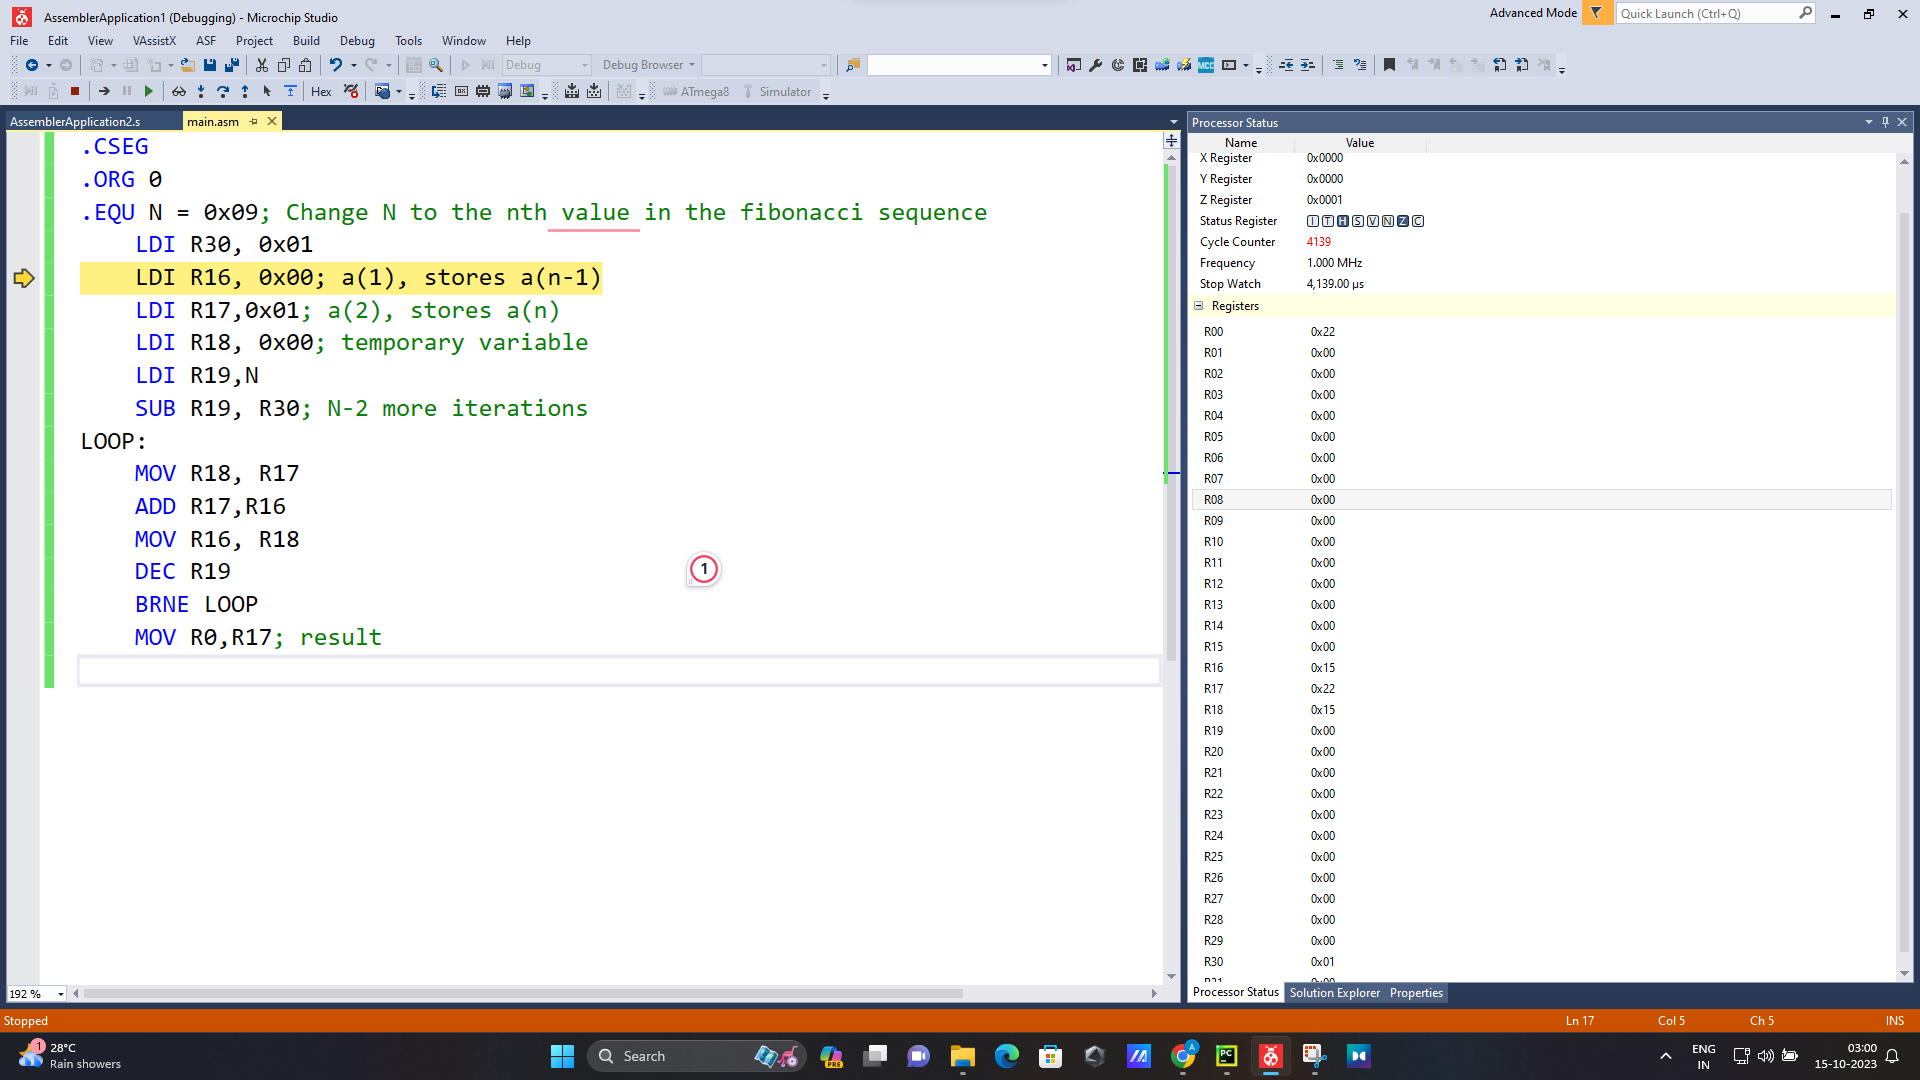
\includegraphics[width=1\linewidth]{prob5.png}
\end{figure}
\captionof{figure}{Screenshot for Problem 5}

\subsection{Inferences}
This assembly code calculates the nth value in the Fibonacci sequence, where the value of n is specified as N. It uses a loop and a set of registers (R16, R17, R18, R19, and R30) to calculate.

\subsubsection{Register Transfers}
\begin{enumerate}
\item Load: LDI, LDS to load data
\item Store: STS to store
\item Move: SUB- Register to Register Moves
\end{enumerate}

\subsubsection{Clock Cycles per Instruction}
\begin{enumerate}
\item LDI: 1 Clock Cycle
\item SUB: 1 Clock Cycle
\item MOV: 1 Clock Cycle
\item MOV: 1 Clock Cycle
\item ADD: 1 Clock Cycle
\item DEC: 1 Clock Cycle
\item Branch Statements: 1 or 2 Clock Cycles depending on result
\end{enumerate}

\subsubsection{Latency}
The latency of this AVR Assembly Code is $6N \mu s$, where $N$ is the number N for which a(N) has to be found

\subsubsection{Throughput}
Throughput of a code is defined as:
$$ Throughput \equiv \frac{\text{Number of Computations(tasks) Done}}{\text{Time Taken}}$$
Here, we define the task to be finding the $N^{th}$ number in the Fibonacci Series

$Throughput= \frac{10^6}{6N}$ Tasks /s

\subsubsection{Limitations}
\begin{enumerate}
\item This code, like the rest, is limited by the size. It can only find $N^{th}$ term as long as it can be stored within 8 bits
\end{enumerate}

\end{document}